\documentclass[aspectratio=169, table]{beamer}

\usepackage{colortbl}
\usepackage{xcolor}
\usepackage{listings}
\usepackage{tikz}
\usetikzlibrary{positioning, arrows.meta, fit, shapes.geometric, positioning}

\usetheme{Pradita}


\usepackage{listings}
\lstdefinestyle{SqlStyle}{
language=SQL,
basicstyle=\ttfamily\footnotesize,
morekeywords={REAL, TEXT, REFERENCES},
keywordstyle=\color{blue},
commentstyle=\color{gray},
stringstyle=\color{red},
breaklines=true,
showstringspaces=false,
tabsize=2,
captionpos=b,
numbers=left,
numberstyle=\tiny\color{gray},
frame=lines,
backgroundcolor=\color{lightgray!10},
comment=[l]{//},
morecomment=[s]{/*}{*/},
commentstyle=\color{gray}\ttfamily,
string=[s]{'}{'},
morestring=[s]{"}{"},
%	stringstyle=\color{teal}\ttfamily,
%	showstringspaces=false
}

\lstdefinelanguage{bash} {
keywords={},
basicstyle=\ttfamily\small,
keywordstyle=\color{blue}\bfseries,
ndkeywords={iex},
ndkeywordstyle=\color{purple}\bfseries,
sensitive=true,
commentstyle=\color{gray},
stringstyle=\color{red},
numbers=left,
numberstyle=\tiny\color{gray},
breaklines=true,
frame=lines,
backgroundcolor=\color{lightgray!10},
tabsize=2,
comment=[l]{\#},
morecomment=[s]{/*}{*/},
commentstyle=\color{gray}\ttfamily,
stringstyle=\color{purple}\ttfamily,
showstringspaces=false
}

% Define Java language style for listings
\lstdefinestyle{JavaScript}{
	language=Java,
	basicstyle=\ttfamily\footnotesize,
	keywordstyle=\color{blue},
	commentstyle=\color{gray},
	stringstyle=\color{red},
	breaklines=true,
	showstringspaces=false,
	tabsize=4,
	captionpos=b,
	numbers=left,
	numberstyle=\tiny\color{gray},
	frame=lines,
	backgroundcolor=\color{lightgray!10},
	comment=[l]{//},
	morecomment=[s]{/*}{*/},
	commentstyle=\color{gray}\ttfamily,
	string=[s]{'}{'},
	morestring=[s]{"}{"},
	%	stringstyle=\color{teal}\ttfamily,
	%	showstringspaces=false
}

\title{\Huge Big Data Processing \\
\vspace{10pt}
Technologies}
\subtitle{IT140704 - Big Data for Business}
%\date[Serial]{Penggunaan Large Language Model untuk Pengajaran}
\author{\textbf{Alfa Yohannis}}
\begin{document}

\frame{\titlepage}


\begin{frame}[fragile]
\frametitle{Contents}
\vspace{20pt}
\begin{columns}[t]
	\column{0.5\textwidth}
	\tableofcontents[sections={1-7}]
	
	\column{0.5\textwidth}
	\tableofcontents[sections={8-20}]
\end{columns}
\end{frame}


\begin{frame}{\hfill}
	\centering
	\Huge{\textbf{Are traditional manual processing approaches sufficient for big data – or are there better approaches available today?}}
\end{frame}





\section{Introduction}

\begin{frame}{Introduction}
	\vspace{20pt}
	
	\begin{itemize}
		\item Big data processing transforms raw data into structured information to support Business Intelligence (BI) and Machine Learning (ML).
		
		\item Processing technologies act as a bridge between data collection and value extraction for strategic decisions and operational efficiency.
		
		\item Data processing determines the effectiveness of integration, cleaning, transformation, and preparation in modern data architecture.
		
		\item This chapter covers:
		\begin{itemize}
			\item Concepts and roles of big data processing in data architecture.
			\item Data flow from sources to data lakes and into warehouses or lakehouses.
			\item Batch and stream processing paradigms for reporting and real-time fraud detection.
			\item Core frameworks like Hadoop MapReduce and Apache Spark.
			\item Ecosystem tools such as Hive, HBase, Sqoop, and Kafka.
			\item Strategic implications for cost, scalability, integration, and organisational skills.
		\end{itemize}
	\end{itemize}
	
\end{frame}

\section{Overview of Big Data Processing}

\begin{frame}{Overview of Big Data Processing}
	\vspace{20pt}
	
	\begin{itemize}
		\item Big data processing transforms large and diverse data into valuable information for organisations.
		
		\item This involves reading, cleaning, integrating, transforming, and analysing data from multiple sources.
		
		\item Technologies used include Hadoop MapReduce, Apache Spark, and other streaming frameworks.
		
		\item The diagram on the next slide shows the data processing architecture, from ingestion to serving for BI and ML.
	\end{itemize}
	
\end{frame}


\begin{frame}{Big Data Processing Architecture}
	\vspace{20pt}
	
	\begin{figure}
		\centering
		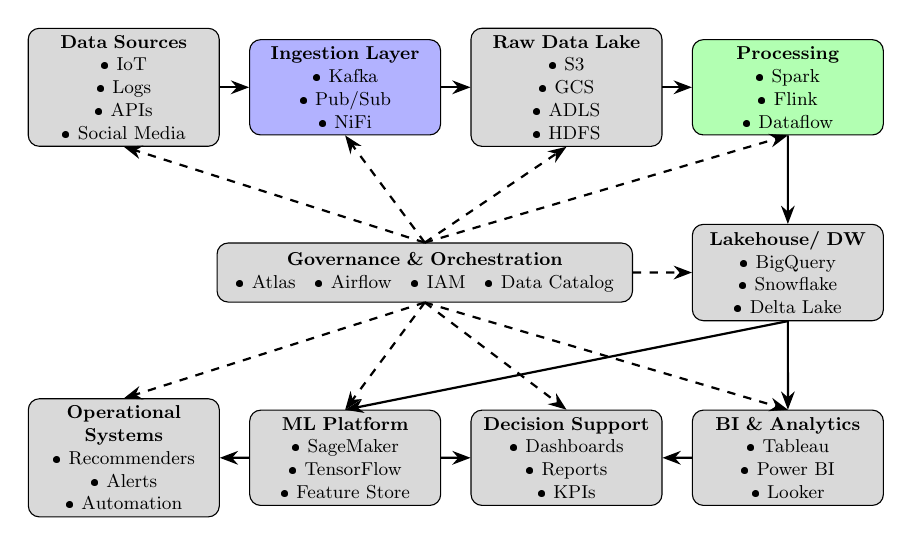
\begin{tikzpicture}[scale=0.75, transform shape, node distance=1cm and 0.5cm]
			
			% Define styles
			\tikzset{
				box/.style={
					rectangle, draw, rounded corners,
					minimum width=2.2cm, minimum height=1cm,
					text width=3cm, align=center, font=\small
				},
				widebox/.style={
					rectangle, draw, rounded corners,
					minimum width=6.5cm, minimum height=1cm,
					text width=6.8cm, align=center, font=\small
				},
				source/.style={box, fill=gray!30},
				ingestion/.style={box, fill=blue!30},
				storage/.style={box, fill=gray!30},
				processing/.style={box, fill=green!30},
				lakehouse/.style={box, fill=gray!30},
				serving/.style={box, fill=gray!30},
				ml/.style={box, fill=gray!30},
				governance/.style={widebox, fill=gray!30},
				output/.style={box, fill=gray!30},
				arrow/.style={thick, ->, >=Stealth},
				dashedarrow/.style={thick, dashed, ->, >=Stealth}
			}
			
			% Main flow (horizontal line)
			\node (source)    [source]        {\textbf{Data Sources}\\• IoT\\• Logs\\• APIs\\• Social Media};
			\node (ingest)    [ingestion, right=of source] {\textbf{Ingestion Layer}\\• Kafka\\• Pub/Sub\\• NiFi};
			\node (lake)      [storage,   right=of ingest] {\textbf{Raw Data Lake}\\• S3\\• GCS\\• ADLS\\• HDFS};
			\node (process)   [processing, right=of lake] {\textbf{Processing}\\• Spark\\• Flink\\• Dataflow};
			
			% Warehouse
			\node (warehouse) [lakehouse, below=1.5cm of process] {\textbf{Lakehouse/ DW}\\• BigQuery\\• Snowflake\\• Delta Lake};
			
			% Governance (above lake and process)
			\node (gov)       [governance, left=1cm of warehouse] {\textbf{Governance \& Orchestration}\\• Atlas\quad• Airflow\quad• IAM\quad• Data Catalog};
			
			% BI and ML 
			\node (bi)        [serving, below=1.5cm of warehouse] {\textbf{BI \& Analytics}\\• Tableau\\• Power BI\\• Looker};
			\node (decision)  [output, left=.5cm of bi] {\textbf{Decision Support}\\• Dashboards\\• Reports\\• KPIs};
			
			\node (ml)        [ml, left= of decision] {\textbf{ML Platform}\\• SageMaker\\• TensorFlow\\• Feature Store};
			\node (opsys)     [output, left=.5cm of ml] {\textbf{Operational Systems}\\• Recommenders\\• Alerts\\• Automation};
			
			% Arrows (main flow)
			\draw[arrow] (source) -- (ingest);
			\draw[arrow] (ingest) -- (lake);
			\draw[arrow] (lake) -- (process);
			\draw[arrow] (process) -- (warehouse);
			
			% BI and ML branches
			\draw[arrow] (warehouse.south) -- (bi.north);
			\draw[arrow] (warehouse.south) -- (ml.north);
			\draw[arrow] (bi) -- (decision);
			\draw[arrow] (ml) -- (opsys);
			\draw[arrow] (ml) -- (decision);
			
			% Governance dashed arrows to all
			\draw[dashedarrow] (gov.north) -- (source.south);
			\draw[dashedarrow] (gov.north) -- (ingest.south);
			\draw[dashedarrow] (gov.north) -- (lake.south);
			\draw[dashedarrow] (gov.north) -- (process.south);
			\draw[dashedarrow] (gov.east) -- (warehouse.west);
			\draw[dashedarrow] (gov.south) --  (bi.north);
			\draw[dashedarrow] (gov.south) --  (ml.north);
			\draw[dashedarrow] (gov.south) --  (decision.north);
			\draw[dashedarrow] (gov.south) --  (opsys.north);
			
		\end{tikzpicture}
		\label{fig:bigdata-processing}
	\end{figure}
	
\end{frame}

\section{Data Ingestion Recap}

\begin{frame}{Data Ingestion Recap}
	\vspace{10pt}
	
	\begin{columns}[T]
		
		\column{0.5\textwidth}
		\begin{itemize}
			\item Data ingestion is the first stage in big data architecture, loading data into a central data lake.
			
			\item Quality and variety of ingested data affect downstream processing and analysis.
			
			\item Common sources include IoT sensors, business apps, social media, log files, transactions, and open data.
		\end{itemize}
		
		\column{0.5\textwidth}
		\begin{itemize}
			\item \textbf{Ingestion methods:}
			\begin{itemize}
				\item Batch: periodic loading.
				\item Streaming: real-time loading.
			\end{itemize}
			
			\item \textbf{Data types ingested:} structured (tables, e.g. transactions), semi-structured (JSON, XML), and unstructured (text, images, videos, audio).
			
			\item Understanding ingestion ensures effective storage and processing strategies for BI and ML.
		\end{itemize}
		
	\end{columns}
	
\end{frame}

\section{Apache Kafka for Real-Time Ingestion}

\begin{frame}{Apache Kafka: Publish-Subscribe Architecture}
	\vspace{10pt}
	
	\begin{figure}
		\centering
		\scalebox{0.85}{
			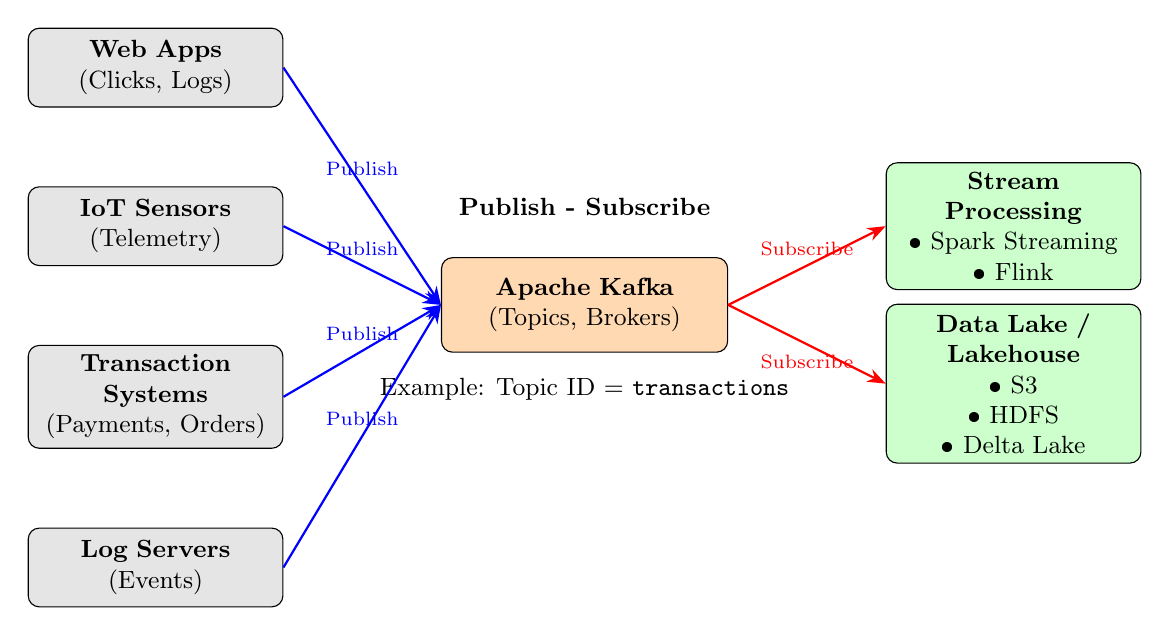
\begin{tikzpicture}[node distance=1cm and 0.8cm]
				
				% Styles
				\tikzset{
					component/.style={
						rectangle, draw, rounded corners,
						minimum width=2.5cm, minimum height=1cm,
						text width=3cm, align=center, font=\small, fill=gray!20
					},
					kafka/.style={
						rectangle, draw, rounded corners,
						minimum width=3.2cm, minimum height=1.2cm,
						text width=3.4cm, align=center, font=\small, fill=orange!30
					},
					consumer/.style={
						rectangle, draw, rounded corners,
						minimum width=2.5cm, minimum height=1cm,
						text width=3cm, align=center, font=\small, fill=green!20
					},
					labelbox/.style={
						draw=none, fill=none, text centered, font=\small
					},
					arrowpub/.style={thick, ->, >=Stealth, blue},
					arrowsub/.style={thick, ->, >=Stealth, red}
				}
				
				% Producers
				\node (webapp) [component] {\textbf{Web Apps}\\(Clicks, Logs)};
				\node (iot) [component, below=of webapp] {\textbf{IoT Sensors}\\(Telemetry)};
				\node (trx) [component, below=of iot] {\textbf{Transaction Systems}\\(Payments, Orders)};
				\node (log) [component, below=of trx] {\textbf{Log Servers}\\(Events)};
				
				% Kafka
				\node (kafka) [kafka, right=2cm of iot, yshift=-1cm] {\textbf{Apache Kafka}\\(Topics, Brokers)};
				
				% Topic ID label
				\node (topic) [labelbox, below=0.2cm of kafka] {Example: Topic ID = \texttt{transactions}};
				
				% Consumers
				\node (stream) [consumer, right=2cm of kafka, yshift=1cm] {\textbf{Stream Processing}\\• Spark Streaming\\• Flink};
				\node (lake) [consumer, right=2cm of kafka, yshift=-1cm] {\textbf{Data Lake / Lakehouse}\\• S3\\• HDFS\\• Delta Lake};
				
				% Publish arrows: producers to kafka
				\draw[arrowpub] (webapp.east) -- node[above, font=\scriptsize, blue] {Publish} (kafka.west);
				\draw[arrowpub] (iot.east) -- node[above, font=\scriptsize, blue] {Publish} (kafka.west);
				\draw[arrowpub] (trx.east) -- node[above, font=\scriptsize, blue] {Publish} (kafka.west);
				\draw[arrowpub] (log.east) -- node[above, font=\scriptsize, blue] {Publish} (kafka.west);
				
				% Subscribe arrows: kafka to consumers
				\draw[arrowsub] (kafka.east) -- node[above, font=\scriptsize, red] {Subscribe} (stream.west);
				\draw[arrowsub] (kafka.east) -- node[below, font=\scriptsize, red] {Subscribe} (lake.west);
				
				% Publish-subscribe label
				\node (pubsub) [labelbox, above=0.4cm of kafka] {\textbf{Publish - Subscribe}};
				
			\end{tikzpicture}
		}
	\end{figure}
	
\end{frame}


\begin{frame}{Apache Kafka for Real-Time Ingestion}
	\vspace{20pt}
	
	\begin{itemize}
		\item \textbf{Apache Kafka} is a streaming platform for high-throughput, low-latency, and scalable data ingestion.
		
		\item Developed by LinkedIn and now open-source under Apache, enabling reliable real-time pipelines.
		
		\item Functions as a \textbf{message broker} with publish-subscribe: producers send data to topics, consumers read as needed.
		
		\item Connects sources like web apps, IoT sensors, transactions, and logs to stream processors (Flink, Spark) or data lakes for batch processing.
		
		\item \textbf{Business uses:}
		\begin{itemize}
			\item Real-time user tracking and recommendations.
			\item Fraud detection in financial transactions.
			\item IoT sensor data for operational control.
		\end{itemize}
		
		\item Supports up-to-date analytics and decisions in big data architectures.
	\end{itemize}
	
\end{frame}

\section{Data Processing in Big Data Architecture}

\begin{frame}{Data Processing in Big Data Architecture}
	\vspace{10pt}
	
	\begin{itemize}
		\item \textbf{Processing} transforms, cleans, integrates, and structures data for effective business analysis and ML.
		
		\item Without processing, data lakes remain raw and lack strategic value.
		
		\item Key activities:
		\begin{itemize}
			\item \textbf{Transform:} convert formats, calculate aggregates, create derived data.
			\item \textbf{Clean:} remove duplicates, handle missing or invalid values.
			\item \textbf{Integrate:} merge data from multiple sources for cross-analysis.
			\item \textbf{Structure:} organise into tables or files for warehouses/lakehouses.
		\end{itemize}
		
		\item \textbf{Warehouse vs Lakehouse:}
		\begin{itemize}
			\item \textbf{Warehouse (ETL):} strict pre-load processing for clean, validated data (finance, compliance, reporting).
			\item \textbf{Lakehouse (ELT):} load raw data first, transform as needed for fast exploration \& ML.
		\end{itemize}
		
		\item Processing impacts data quality, speed, flexibility, and scalability for strategic decisions.
	\end{itemize}
	
\end{frame}

\begin{frame}{Batch vs Stream Processing}
	\vspace{10pt}
	
	\begin{columns}[T]
		\column{0.5\textwidth}
		\textbf{Batch Processing}
		\vspace{5pt}
		\begin{itemize}
			\item Processes large data collected over time in one run.
			\item For non-urgent tasks: finance reports, sales summaries, trends.
			\item Uses MapReduce, Spark batch.
			\item Fits warehouses needing clean, validated data.
			\item Example: banks generate daily/monthly reports off-hours.
		\end{itemize}
		
		\column{0.5\textwidth}
		\textbf{Stream Processing}
		\vspace{5pt}
		\begin{itemize}
			\item Processes data instantly on arrival.
			\item Ideal for fast-response: fraud detection, IoT, recommendations.
			\item Uses Kafka Streams, Flink, Spark Streaming.
			\item Fits lakehouse/hybrid for real-time analytics/ML.
			\item Example: detects fraud within seconds of a transaction.
		\end{itemize}
		
	\end{columns}
	
	\vspace{5pt}
	Understanding both ensures pipelines support timely decisions.
	
\end{frame}

\section{Hadoop Ecosystem}

\begin{frame}{Introduction to Hadoop}
	\vspace{10pt}
	
	\begin{itemize}
		\item Hadoop is a core big data technology enabling efficient, low-cost storage and processing of massive datasets.
		
		\item Inspired by Google File System and MapReduce, now an Apache project.
		
		\item \textbf{Main components:}
		\begin{itemize}
			\item \textbf{HDFS:} distributed file system splitting large files into blocks across nodes with replication for reliability.
			\item \textbf{MapReduce:} parallel processing model operating near data to minimise transfer costs.
		\end{itemize}
		
		\item Scalable, fault-tolerant, handling petabytes of diverse data by adding nodes easily.
		
		\item Includes tools like Hive, HBase, Pig, and Sqoop for integration, querying, and analytics.
		
		\item Hadoop is a foundation of modern big data for batch processing, business analysis, and strategic decisions.
	\end{itemize}
	
\end{frame}

\section{MapReduce}
\begin{frame}{MapReduce Workflow}
	\vspace{10pt}
	
	\begin{figure}
		\centering
		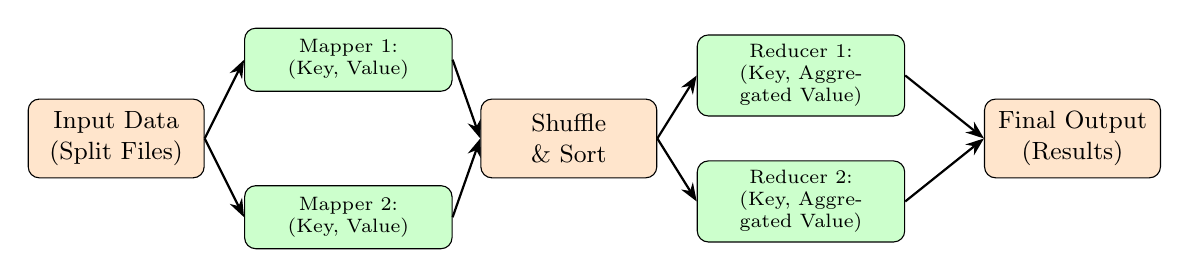
\begin{tikzpicture}[node distance=0.5cm and 0.5cm, scale=1, transform shape]
			
			% Styles
			\tikzset{
				stage/.style={
					rectangle, draw, rounded corners,
					minimum width=2cm, minimum height=1cm,
					text width=2cm, align=center, font=\small, fill=orange!20
				},
				process/.style={
					rectangle, draw, rounded corners,
					minimum width=2.2cm, minimum height=0.8cm,
					text width=2.4cm, align=center, font=\scriptsize, fill=green!20
				},
				arrow/.style={thick, ->, >=Stealth}
			}
			
			% Input data
			\node (input) [stage] {Input Data\\(Split Files)};
			
			% Mappers
			\node (map1) [process, right=of input, yshift=1cm] {Mapper 1:\\(Key, Value)};
			\node (map2) [process, right=of input, yshift=-1cm] {Mapper 2:\\(Key, Value)};
			
			% Shuffle and Sort
			\node (shuffle) [stage, right=3.5cm of input] {Shuffle \& Sort};
			
			% Reducers
			\node (reduce1) [process, right=of shuffle, yshift=0.8cm] {Reducer 1:\\(Key, Aggregated Value)};
			\node (reduce2) [process, right=of shuffle, yshift=-0.8cm] {Reducer 2:\\(Key, Aggregated Value)};
			
			% Output
			\node (output) [stage, right=of reduce1, xshift=0.5cm, yshift=-0.8cm] {Final Output\\(Results)};
			
			% Arrows: Input to Mappers
			\draw[arrow] (input.east) -- (map1.west);
			\draw[arrow] (input.east) -- (map2.west);
			
			% Arrows: Mappers to Shuffle
			\draw[arrow] (map1.east) -- (shuffle.west);
			\draw[arrow] (map2.east) -- (shuffle.west);
			
			% Arrows: Shuffle to Reducers
			\draw[arrow] (shuffle.east) -- (reduce1.west);
			\draw[arrow] (shuffle.east) -- (reduce2.west);
			
			% Arrows: Reducers to Output
			\draw[arrow] (reduce1.east) -- (output.west);
			\draw[arrow] (reduce2.east) -- (output.west);
			
		\end{tikzpicture}
	\end{figure}
	
\end{frame}

\begin{frame}{Concept and Benefits of MapReduce}
	\vspace{20pt}
	
	\begin{itemize}
		\item \textbf{Concept:} splits input data into chunks processed in parallel (Map) to produce key-value pairs, then aggregates by key (Reduce) for integrated results across nodes.
		
		\item \textbf{Benefits:}
		\begin{itemize}
			\item Handles petabyte-scale batch processing efficiently.
			\item Scalable by adding nodes to the cluster.
			\item Fault-tolerant with automatic task rescheduling.
			\item Optimises data locality, processing data near its storage to reduce transfer costs.
		\end{itemize}
		
		\item \textbf{Limitations:}
		\begin{itemize}
			\item Programming is complex compared to SQL.
			\item Not suitable for real-time or near real-time analytics due to high batch latency.
		\end{itemize}
		
		\item \textbf{Use case:} ideal for large-scale batch tasks such as historical data aggregation and periodic reporting, but less flexible for interactive or real-time analytics.
	\end{itemize}
	
\end{frame}

\begin{frame}{MapReduce for Data Warehouse Preparation}
	\vspace{20pt}
	
	MapReduce plays a key role in preparing large data sets for warehouses. Two major business use cases are:
	
	\begin{itemize}
		\item \textbf{Retail transaction aggregation:} supermarkets and e-commerce platforms generate millions of daily sales records stored in distributed POS systems. MapReduce combines these by product category, region, or date to load into warehouses for sales analysis, inventory optimisation, promotions, and strategic purchasing.
		
		\item \textbf{Log summarisation for compliance reporting:} financial and telecom firms must keep detailed system and transaction logs for audits and regulation. MapReduce parses raw logs, extracts relevant fields, groups by activity or user, and produces summaries needed for compliance reporting.
	\end{itemize}
	
	This ensures data entering warehouses is structured, clean, and ready for reporting, BI, and strategic decisions.
	
\end{frame}

\section{Frameworks and Tools in Hadoop Ecosystem}
\begin{frame}{Frameworks \& Tools in the Hadoop Ecosystem}
	\vspace{20pt}
	
	Hadoop is not a standalone tool; it has an ecosystem of frameworks and tools that enhance its capabilities. The figure below shows some key frameworks and their contributions within the Hadoop ecosystem, \textbf{but is not limited to these}.
	
	\begin{figure}
		\centering
		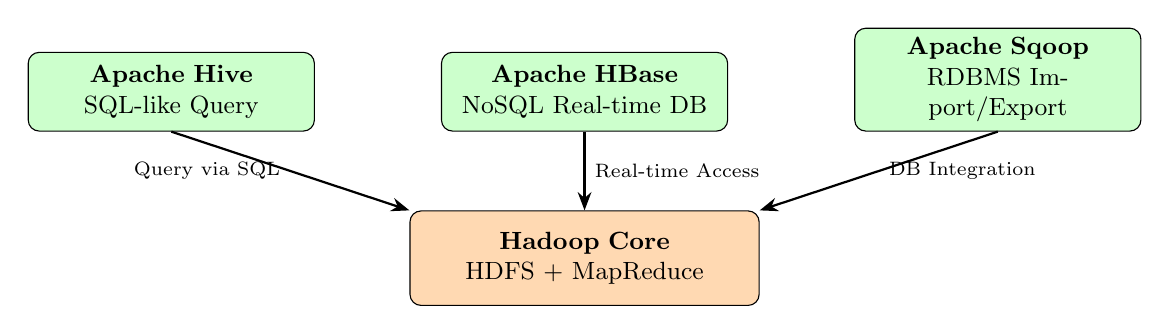
\begin{tikzpicture}[node distance=1cm and 1.2cm]
			
			% Styles
			\tikzset{
				core/.style={
					rectangle, draw, rounded corners,
					minimum width=4cm, minimum height=1.2cm,
					text width=4.2cm, align=center, font=\small, fill=orange!30
				},
				component/.style={
					rectangle, draw, rounded corners,
					minimum width=3.2cm, minimum height=1cm,
					text width=3.4cm, align=center, font=\small, fill=green!20
				},
				arrow/.style={thick, ->, >=Stealth},
				labelbox/.style={
					draw=none, fill=none, text centered, font=\small
				}
			}
			
			% Hadoop Core
			\node (core) [core] {\textbf{Hadoop Core}\\HDFS + MapReduce};
			
			% Components above
			\node (hive) [component, above left=of core] {\textbf{Apache Hive}\\SQL-like Query};
			\node (hbase) [component, above=of core] {\textbf{Apache HBase}\\NoSQL Real-time DB};
			\node (sqoop) [component, above right=of core] {\textbf{Apache Sqoop}\\RDBMS Import/Export};
			
			% Arrows with labels
			\draw[arrow] (hive.south) -- node[left, font=\scriptsize] {Query via SQL} (core.north west);
			\draw[arrow] (hbase.south) -- node[right, font=\scriptsize] {Real-time Access} (core.north);
			\draw[arrow] (sqoop.south) -- node[right, font=\scriptsize] {DB Integration} (core.north east);
			
		\end{tikzpicture}
		\label{fig:hadoop-ecosystem-complete}
	\end{figure}
	
\end{frame}

\begin{frame}{Apache Hive}
	\vspace{20pt}
	
	\begin{itemize}
		\item Apache Hive is a key Hadoop tool enabling SQL-like queries on HDFS data.
		\item Developed by Facebook in 2008 to simplify MapReduce programming.
		\item Translates HiveQL commands into MapReduce, Tez, or Spark jobs executed across Hadoop clusters.
		\item Allows analysts to analyse large datasets using familiar SQL syntax.
		\item Benefits:
		\begin{itemize}
			\item Speeds up Hadoop adoption.
			\item Reduces technical training needs.
			\item Integrates Hadoop with BI tools via standard SQL connections.
		\end{itemize}
	\end{itemize}
	
\end{frame}

\begin{frame}{Apache HBase and Sqoop}
	\vspace{20pt}
	
	\begin{itemize}
		\item \textbf{Apache HBase:}
		\begin{itemize}
			\item Distributed NoSQL DB on HDFS with fast read-write for massive data.
			\item Uses key-value model similar to Google BigTable.
			\item Supports real-time lookups, e.g. telcos storing user usage data for quick analysis.
			\item Complements Hadoop batch processing with real-time database capability.
		\end{itemize}
		\item \textbf{Apache Sqoop:}
		\begin{itemize}
			\item Imports/exports data between Hadoop and RDBMS (MySQL, Oracle) via MapReduce jobs.
			\item Enables fast parallel data transfer.
			\item Used to export processed data to RDBMS or import historical data to Hadoop for analysis.
			\item Enhances interoperability with existing enterprise systems.
		\end{itemize}
	\end{itemize}
	
\end{frame}

\section{Apache Spark}
\begin{frame}{Introduction to Apache Spark}
	\vspace{20pt}
	
	\begin{itemize}
		\item Apache Spark is a big data framework overcoming MapReduce’s speed and flexibility limits.
		
		\item Developed at UC Berkeley AMPLab (2009), open-sourced under Apache in 2014.
		
		\item Uses in-memory processing to avoid disk I/O bottlenecks, running 10–100x faster than MapReduce.
		
		\item Supports batch, streaming (Spark Streaming), machine learning (MLlib), and graph processing (GraphX).
		
		\item Enables real-time analytics and recommendations, e.g. analysing customer behaviour instantly.
		
		\item Provides APIs in Java, Python, and R for easy integration and rapid development.
		
		\item Its speed, scalability, and multi-workload support make Spark widely adopted in modern big data.
	\end{itemize}
	
\end{frame}


\section{Spark SQL}
\begin{frame}{Spark SQL}
	\vspace{20pt}
	
	\begin{itemize}
		\item Spark SQL enables SQL queries on data from HDFS, Hive, JSON, Parquet, JDBC, and more.
		
		\item Bridges SQL familiarity with Spark’s distributed, in-memory processing.
		
		\item Queries compile into Spark execution plans for fast, scalable performance.
		
		\item Supports DataFrame and Dataset APIs optimised by Catalyst Optimizer.
		
		\item Used in ETL pipelines to read, clean, transform data, and load into warehouses or Delta Lake.
		
		\item Provides analytics-ready data for BI and data science using familiar SQL.
		
		\item Example: Fintech firms transform daily transactions for compliance reporting efficiently.
	\end{itemize}
	
\end{frame}

\section{Business Case 1}
\begin{frame}{\LARGE{Batch Processing for Financial Data Warehouse}}
	\vspace{20pt}
	
	\textbf{Context.} Banks generate millions of transactions daily from ATMs, mobile banking, interbank transfers, and merchant payments. This data resides in different operational systems with varied formats and must be consolidated into structured warehouses for reporting, audit, and risk analysis.
	
	\vspace{10pt}
	\textbf{Technology.} Hadoop MapReduce or Spark batch processing performs large-scale ETL: extracting data, cleaning duplicates or anomalies, transforming into standard reporting schemas, and loading into SQL-based warehouses. Spark SQL is often used to accelerate transformations and aggregations.
	
	\vspace{10pt}
	\textbf{Impact.} Enables timely financial reports for regulators, supports profitability analysis, customer segmentation, and credit risk assessments with complete and reliable data.
	
\end{frame}

\section{Business Case 2}
\begin{frame}{Stream Processing for Near Real-Time ODS}
	\vspace{20pt}
	
	Stream processing builds near real-time \textbf{Operational Data Stores} (ODS) for instant analytics and operations.
	
	\vspace{10pt}
	\textbf{Context.} An e-commerce platform processes millions of user clicks, searches, purchases, and stock updates per minute to power instant recommendations, real-time fraud detection, and operational dashboards.
	
	\vspace{10pt}
	\textbf{Technology.} Uses Apache Kafka for ingestion, Spark Streaming or Flink for real-time processing, and NoSQL stores like HBase or in-memory DBs like Redis for low-latency access.
	
	\vspace{10pt}
	\textbf{Business Impact.} Enables transaction anomaly detection in seconds, real-time personalised recommendations to boost sales, and live dashboards for rapid business decisions during campaigns.
	
\end{frame}


\section{Strategic Implications}
\begin{frame}{Strategic Implications for Business}
	\vspace{20pt}
	
	Big data processing technologies like Hadoop, Spark, and Kafka have strategic impacts.
	
	\vspace{10pt}
	First, they enable \textbf{faster decision-making}. Organisations gain near real-time insights to make timely, data-driven decisions.
	
	\vspace{10pt}
	Second, they deepen \textbf{customer insights}. Streaming analytics allows instant behaviour analysis for personalised offers, increasing loyalty and revenue.
	
	\vspace{10pt}
	Third, adoption offers a \textbf{competitive advantage} through innovation, operational efficiency, and agile market response.
	
	\vspace{10pt}
	However, costs for infrastructure, skilled teams, and integration need consideration to ensure scalability and optimal performance.
	
\end{frame}

\section{Conclusion}
\begin{frame}{Conclusion}
	\vspace{20pt}
	
	\begin{itemize}
		\item This chapter covered \textbf{big data processing concepts and technologies}: data ingestion, batch vs stream processing, Hadoop MapReduce, Apache Spark, and ecosystem tools like Hive, HBase, Sqoop, and Kafka.
		
		\item \textbf{Big data processing transforms} raw, unstructured data into structured, analysis-ready formats for business intelligence, machine learning, and operational analytics.
		
		\item Mastering these technologies \textbf{enables organisations} to build scalable data architectures that generate insights and support fast, data-driven decisions.
		
		\item \textbf{Choosing the right} technologies, with skilled teams, is key for successful digital transformation and gaining competitive advantage in the data-driven economy.
	\end{itemize}
	
\end{frame}




\end{document}
